\documentclass[tikz]{standalone} 
% change to font used in beamer
%\renewcommand{\familydefault}{\sfdefault}

\usetikzlibrary{patterns}

\begin{document}
	
	%\tdplotsetmaincoords{0}{0}
	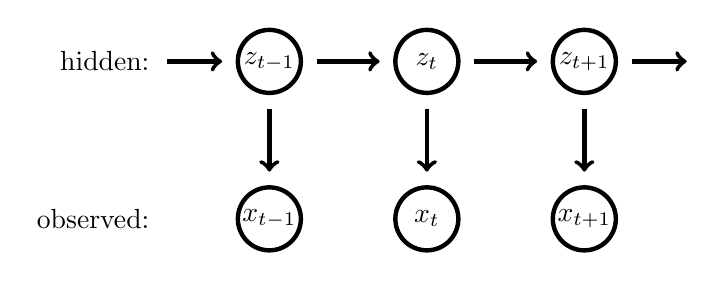
\begin{tikzpicture}[scale=2]
		
		%\draw[] (-0.85,0) node{...};
		\draw[ultra thick,->] (-0.65,0) to (-0.3,0);
		
		\draw[ultra thick,fill=white] (0,0) circle (0.2) node[]{$z_{t-1}$};
		\draw[ultra thick,->] (0.3,0) to (0.7,0);
		
		\draw[ultra thick,fill = white] (1,0) circle (0.2) node[]{$z_t$};
		\draw[ultra thick,->] (1.3,0) to (1.7,0);
		
		\draw[ultra thick,fill = white] (2,0) circle (0.2) node[]{$z_{t+1}$};
		\draw[ultra thick,->] (2.3,0) to (2.65,0);
		
		%\draw[] (3.85,0) node{...};
		
		\draw[ultra thick,fill=white] (0,-1) circle (0.2) node[]{$x_{t-1}$};
		\draw[ultra thick,->] (0,-0.3) to (0,-0.7);
		\draw[ultra thick,fill = white] (1,-1) circle (0.2) node[]{$x_t$};
		\draw[ultra thick,->] (1,-0.3) to (1,-0.7);
		\draw[ultra thick,fill = white] (2,-1) circle (0.2) node[]{$x_{t+1}$};
		\draw[ultra thick,->] (2,-0.3) to (2,-0.7);
		
		\draw[] (-0.7,0) node[left]{hidden:};
		\draw[] (-0.7,-1) node[left]{observed:};
		
	\end{tikzpicture}
	
\end{document}